\documentclass[aspectratio=1610,14pt,t]{beamer}

% Colors
\usepackage{color}
\definecolor{mainorange}{HTML}{EC811B}
\definecolor{lightgrey}{HTML}{888888}

% Syntax highlighting
\usepackage{minted}
\usepackage{alltt}
\newcommand\hi[1]{{\color{mainorange} \textbf{#1}}}

% Theme
\usetheme[%
	subsectionpage=progressbar,
	numbering=fraction,
	progressbar=foot,
]{metropolis}

% Customization
\setbeamertemplate{section in toc}[sections numbered]
\setbeamerfont{title}{size=\fontsize{30}{30}}
\setbeamerfont{block title}{size=\large}
\newcommand\sep{\textcolor{lightgrey}{\rule{\linewidth}{0.05mm}}}

% Positioning
% https://tex.stackexchange.com/a/34929/13059
\def\Put(#1,#2)#3{\leavevmode\makebox(0,0){\put(#1,#2){#3}}}

% Meta
\title{Calling Rust from C and Java}
\date{2017-10-31}
\author{Danilo Bargen (@dbrgn)}
\institute{Rust Zürichsee Meetup}

\begin{document}

\pgfdeclareimage[width=\paperwidth]{bg}{background-dark.pdf}
\usebackgroundtemplate{\pgfuseimage{bg}}
\maketitle

% ----------------------------------------------------------------- %

\begin{frame}[plain,noframenumbering]
	\frametitle{Outline}
	\setcounter{tocdepth}{1}
	\tableofcontents
\end{frame}

% ----------------------------------------------------------------- %

\pgfdeclareimage[width=\paperwidth]{bg}{background-light.pdf}
\usebackgroundtemplate{\pgfuseimage{bg}}

\section{FFI}

\begin{frame}[c]{What is FFI?}
	FFI stands for <<Foreign Function Interface>>.

  It's a way to call functions written in one programming language
  from another one.
\end{frame}

\begin{frame}[c]{How does it work?}
  FFI works if there are known binary calling conventions that both sides adhere to.

  Think of it as a <<communication protocol>>.

  Not all languages have fixed calling conventions. C does, C++ does not.
\end{frame}

\begin{frame}[c]{FFI Is Easy!!!...?}
  Most FFI examples / intros do something like adding two integers.

  That is a totally useless example, since reality is much more complex.

  Biggest pain point once you get started: Heap allocations and pointers.
\end{frame}

\begin{frame}[c]{Memory Ownership}
  If you know Rust, you have probably acquired an intuitive understanding of the
  concept called <<Memory Ownership>>.

  The owner of an object owns its memory.
\end{frame}

\begin{frame}[c]{Let's Talk About Boxes}
  \centering
  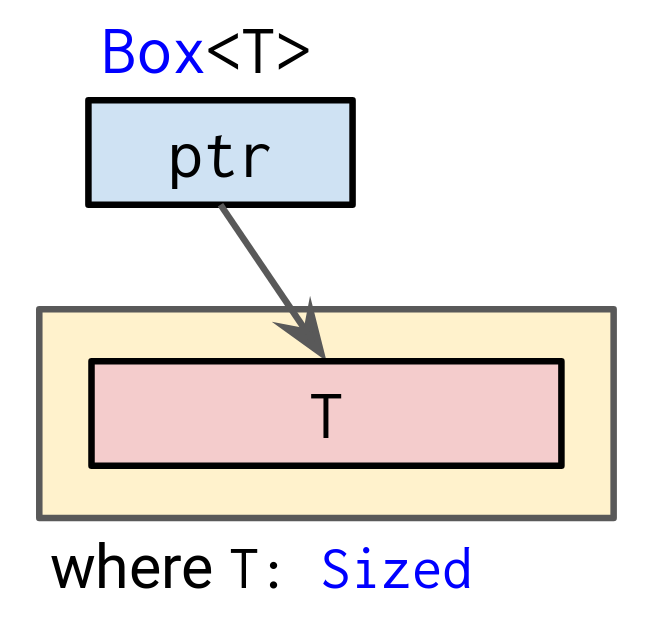
\includegraphics[width=.5\textwidth]{img/box.png}
\end{frame}

\begin{frame}[c]{Here Be Dragons}
    Rust ownership guarantees only cover memory allocated by Rust. For all
    other memory, we cannot make any assumptions.

  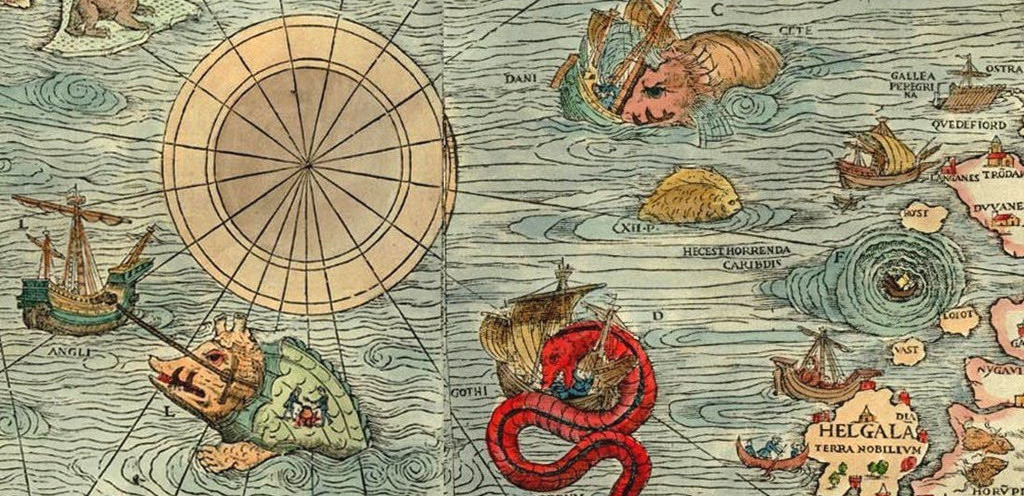
\includegraphics[width=\textwidth]{img/dragons.jpg}
\end{frame}

\begin{frame}[c]{Rust: Beware the Drop}
  \begin{center}
  
\includegraphics[width=.5\textwidth]{img/dragon1.jpg}
  \end{center}

  When returning raw (unsafe) pointers from Rust, remember that the memory owned
  by Rust will be freed when the corresponding value is dropped.
\end{frame}

\begin{frame}[c]{C: Beware Other Allocators}
  \begin{center}
  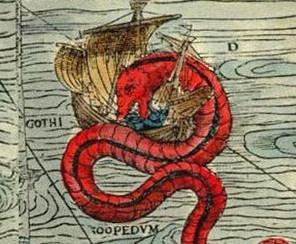
\includegraphics[width=.3\textwidth]{img/dragon2.jpg}
  \end{center}

  By default, Rust uses the jemalloc memory allocator and C does not.

  When handling memory allocated by Rust, do not try to free it in a C program.
\end{frame}

\begin{frame}[c]{Java: Beware the GC}
  \begin{center}
  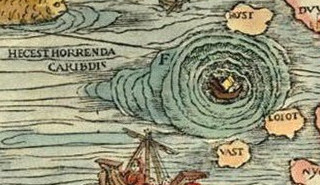
\includegraphics[width=.4\textwidth]{img/dragon3.jpg}
  \end{center}

  When holding on to a Java reference in Rust, the Java runtime must be notified
  about that. Otherwise the memory may be collected by the garbage collector.
\end{frame}

\begin{frame}[c]{It's Dangerous}
  \begin{center}
  
\includegraphics[width=.7\textwidth]{img/dangerous.png}

  \url{doc.rust-lang.org/nomicon/ffi.html}

  \url{jakegoulding.com/rust-ffi-omnibus/}

  \url{valgrind.org/}
  \end{center}
\end{frame}

\section{Parsing ICE Candidates}

\begin{frame}[c]{ICE Candidate Parsing}
  In order to have a practical example in this talk, we'll take a look at a
  simple library I've written.

  That library is a parser for ICE candidates with bindings for C and Java.

  Source: {\small \url{https://github.com/dbrgn/candidateparser}}
\end{frame}

\begin{frame}[c]{WTF are ICE Candidates?}
  \center
  
\includegraphics[width=.5\textwidth]{img/ice-skater.jpg}
\end{frame}

\begin{frame}[c]{WTF are ICE Candidates?}
  \begin{columns}[T]
    \begin{column}{.3\textwidth}
      
\includegraphics[width=\textwidth]{img/ice-skater.jpg}
    \end{column}
    \begin{column}{.7\textwidth}
      No, not that ice.

      \vspace{1em}

      \pause
      ICE stands for <<Interactive Connectivity Establishment>>.

      \vspace{1em}

      It's a protocol used in peer-to-peer networks to establish a connection.
    \end{column}
  \end{columns}
\end{frame}

\begin{frame}[c,fragile]{WTF are ICE Candidates?}
  This is what an ICE candidate looks like:

  \begin{minted}{rust}
candidate:842163049 1 udp 1686052607
1.2.3.4 46154 typ srflx
raddr 10.0.0.17 rport 46154 generation 0
ufrag EEtu network-id 3 network-cost 10
  \end{minted}
\end{frame}

\begin{frame}[c,fragile]{Parsing}
  Since this talk is about FFI, I won't cover the parsing in detail.

  The parser is written in Rust using
  nom\footnote{\url{https://crates.io/crates/nom}}.
  It provides a single function as entry point:

  \begin{minted}[fontsize=\small]{rust}
pub fn parse(sdp: &[u8]) -> Option<IceCandidate>
  \end{minted}
\end{frame}

\begin{frame}[c,fragile]{IceCandidate struct}

  This is the type returned by the parsing function:

  \begin{minted}[fontsize=\footnotesize]{rust}
pub struct IceCandidate {
    pub foundation: String,
    pub component_id: u32,
    pub transport: Transport,
    pub priority: u64,
    pub connection_address: IpAddr,
    pub port: u16,
    pub candidate_type: CandidateType,
    pub rel_addr: Option<IpAddr>,
    pub rel_port: Option<u16>,
    pub extensions: Option<HashMap<Vec<u8>, Vec<u8>>>,
}
  \end{minted}

  \Put(165, 360){
\includegraphics[height=1.4cm]{img/alloc.png}}
  \Put(175, 305){
\includegraphics[height=1.4cm]{img/unknown.png}}
  \Put(205, 250){
\includegraphics[height=1.4cm]{img/unknown.png}}
  \Put(220, 195){
\includegraphics[height=1.4cm]{img/unknown.png}}
  \Put(220, 165){
\includegraphics[height=1.4cm]{img/unknown.png}}
  \Put(310, 110){
\includegraphics[height=1.4cm]{img/alloc.png}}
\end{frame}

\begin{frame}[c,fragile]{Enums}
  Inside the \texttt{IceCandidate} struct, two enums are being used.

  \begin{minted}[fontsize=\small]{rust}
pub enum CandidateType {
  Host, Srflx, Prflx, Relay, Token(String)
}
  \end{minted}

  \begin{minted}[fontsize=\small]{rust}
pub enum Transport {
  Udp, Extension(String)
}
  \end{minted}

  Note that both of them contain associated data.

  \Put(275, 320){
\includegraphics[height=1.3cm]{img/alloc.png}}
  \Put(150, 200){
\includegraphics[height=1.3cm]{img/alloc.png}}
\end{frame}

\begin{frame}[c,fragile]{External Types}

  The \texttt{connection\_address} and the \texttt{rel\_addr} keys contain an
  \texttt{std::net::IpAddr}.

  \begin{minted}[fontsize=\small]{rust}
pub enum IpAddr {
    V4(Ipv4Addr),
    V6(Ipv6Addr),
}
  \end{minted}

  \Put(130, 155){
\includegraphics[height=1.3cm]{img/unknown.png}}
  \Put(130, 120){
\includegraphics[height=1.3cm]{img/unknown.png}}
\end{frame}

\begin{frame}[c,fragile]{Other Complex Types}

  The \texttt{extensions} key type:

  \vspace{3em}

  \texttt{Option<HashMap<Vec<u8>, Vec<u8>>>}.

  \Put(80, 110){
\includegraphics[height=1.3cm]{img/alloc.png}}
  \Put(140, 105){
\includegraphics[height=1.3cm]{img/alloc.png}}
  \Put(215, 105){
\includegraphics[height=1.3cm]{img/alloc.png}}
\end{frame}

\section{Rust $\rightleftharpoons$ C}

\section{Rust $\rightleftharpoons$ Java}

\section{Questions?}


% ----------------------------------------------------------------- %

{
\setbeamertemplate{footline}{}
\pgfdeclareimage[width=\paperwidth]{bg}{background-inverted.pdf}
\usebackgroundtemplate{\pgfuseimage{bg}}
\begin{frame}[standout]
	\begin{centering}
	{\Huge Thank you!}\\
	{\normalsize \url{www.coredump.ch}}\\
	\end{centering}
\end{frame}
}

\end{document}
